\chapter{Conclusiones y trabajos futuros}
\section{Conclusiones.}
Tras el completo estudio del método de Laplace, junto a la experimentación realizada, podemos concluir que es un método consistente y fiable para la determinación sobre cuerpos cercanos aún solo utilizando tres observaciones. Pero hemos comprobado que conforme aumenta la distancia, se dispara el error de la aproximación realizada. Es entendible que el método laplaciano no estuviera optimizado para cuerpos lejanos, pues con los telescopios rudimentarios con los que se trabajaba en aquella época no llegarían a observar más allá del cinturón de asteroides (salvo para objetos más masivos, como Júpiter o Saturno).\\

Hoy día disponemos de mejor tecnología y podemos observar cuerpos más lejanos, pero aún así el método de Laplace no funciona con ellos de manera óptima. Conviene preguntarse, ¿de dónde viene el error al intentar aproximar la órbita de estos? Recordemos las ecuaciones para calcular $r$ y $\rho$ \eqref{eq:triangle_relations_2}.
\[
\left\{
\begin{array}{l}
	\rho=R\ddfrac{\sin{(\psi+\phi)}}{\sin{\phi}}\\
	r=R\ddfrac{\sin{\psi}}{\sin{\phi}}
\end{array}
\right.
\]

Tomando los valores de $r$ y $\rho$ como funciones en $\phi$, podemos deducir rápidamente que éstas divergerán conforme lleguen a 0. Veamos una gráfica con las dos funciones para apreciar mejor cuál es su comportamiento.
\begin{figure}[H]
\centering
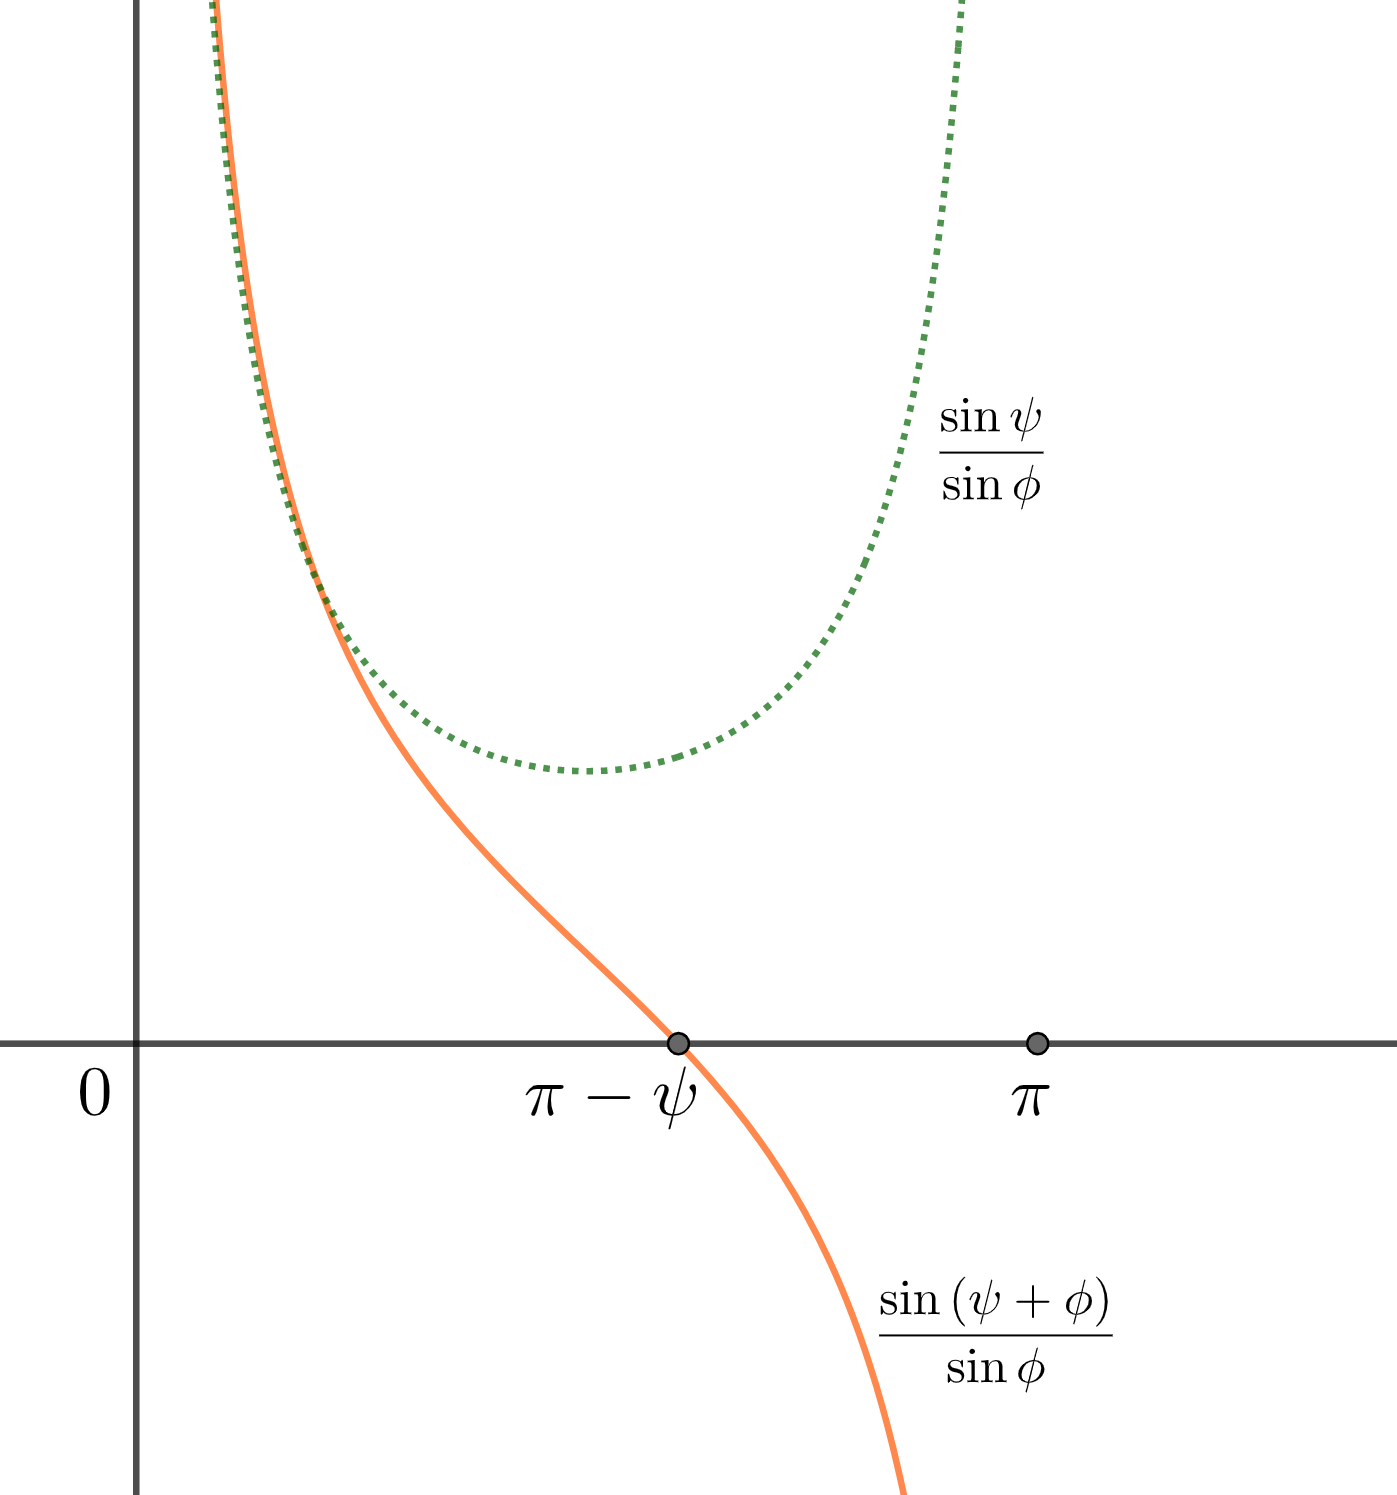
\includegraphics[scale=0.15]{images/motivo_error.png}
\end{figure}

El hecho de que $r=R\ddfrac{\sin{\psi}}{\sin{\phi}}$ diverja en $\pi$ no nos importará, pues el valor de $\phi$ para que sea solución del problema físico ha de ser menor que $\pi-\psi$.\\

Por otra parte, podemos ver en la siguiente figura, cuanto mayor sea la distancia del cuerpo $C$ a la Tierra, menor será el ángulo $\phi$ que forma.
\begin{figure}[H]
\centering
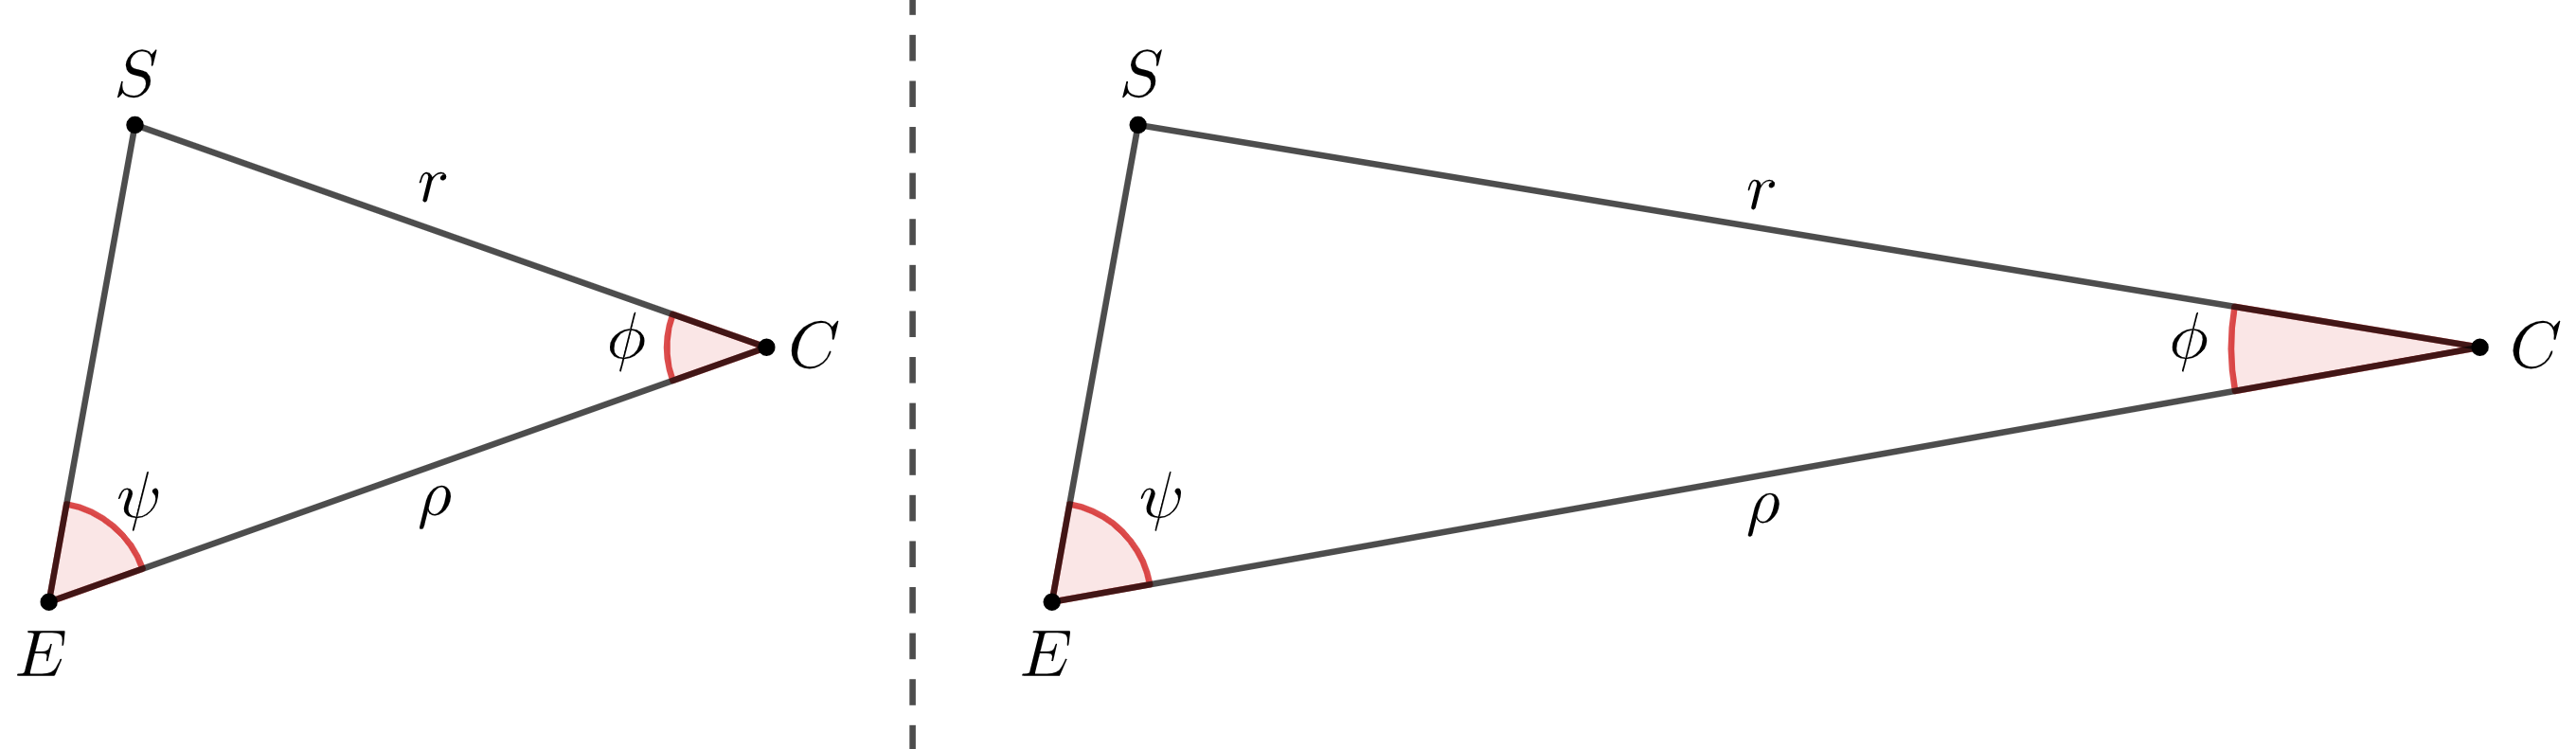
\includegraphics[scale=0.125]{images/bigger_rho_smaller_phi.png}
\caption{Comparación de la variación en el ángulo $\phi$ en función de la distancia $\rho$.}
\label{fig:bigger_rho_smaller_phi.png}
\end{figure}

Con toda esta información podemos proceder de manera similar a como hicimos al final de \ref{sec:neowise}: para que el valor de $\rho$ sea grande, $\phi$ ha de ser pequeño, y cuanto menor sea el valor de $\phi$ mayor impacto tendrá el error en el cálculo de $\rho$ por el hecho de que $\phi$ diverge en 0. Al igual que con el valor de $\rho$ podemos proceder con el valor de $r$.\\

Nótese que el hecho de que el ángulo $\phi$ sea pequeño no tiene que venir de que la distancia de $E$ a $C$ sea grande. Puede darse el caso de que, observando un objeto medianamente cercano, el ángulo $\measuredangle{ESC}$, es decir, el formado en el Sol entre $E$ y $C$, sea cercano a $\pi$ de manera que $\psi$ y $\phi$ serían muy pequeños, induciendo a un mayor error en el cálculo de $\rho$ y $r$. En este caso, sería una buena decisión esperar a un momento próximo para realizar las mediciones.\\

En cuanto a las conclusiones subjetivas que puedo sacar de este trabajo, el estudio sobre la determinación de órbitas me ha parecido realmente interesante y me ha servido para mejorar mi capacidad a la hora de entender un libro de matemáticas desde cero. Además, el hecho de realizar la interfaz gráfica me ha ayudado a aprender a utilizar \textit{Tkinter}, una buena herramienta para implementar GUIs sobre código Python, así como seguir mejorando mi nivel de éste lenguaje de programación.\\

\section{Trabajos futuros.}
Durante toda esta memoria se han ido enumerando diferentes objetivos que podemos ver a continuación:
\begin{itemize}
\item Objetivo 1: repaso de la mecánica celeste.
\item Objetivo 2: pasos para determinar la posición y velocidad de un cuerpo a partir de tres observaciones (método de Laplace).
\item Objetivo 3: obtener las coordenadas astronómicas a partir de la posición y velocidad de un cuerpo.
\item Objetivo 4: estudio del número de soluciones del método de determinación.
\item Objetivo 5: elección de las herramientas para desarrollar el software de determinación.
\item Objetivo 6: implementación de un código que sea capaz de determinar la posición y velocidad mediante el método de Laplace.
\item Objetivo 7: desarrollo de una interfaz gráfica para la determinación de órbitas.
\item Objetivo 8: estudio de la eficacia del método de Laplace.
\end{itemize}

Todos estos objetivos, algunos obligatorios y otros opcionales, han sido cumplidos durante el desarrollo de este trabajo. Sin embargo, aún podemos seguir extendiendo el estudio de la determinación y la implementación del software.\\

Por la parte matemática, se puede continuar desarrollando el método de Laplace estudiando la aproximación de las derivadas utilizando 4 o más observaciones, o cómo utilizar una cuarta observación en el caso de una solución doble. También se puede extender el análisis de los determinantes $D$, $D_1$, $D_2$ y en qué momento desaparecen, para seguir acotando los valores que toman $m$ y $M$ en la ecuación \eqref{eq:phi_solution}. Además, Laplace desarrolló procedimientos con los que mejorar los valores de la posición y velocidad tras aplicar su método mediante el uso de las derivadas de $(\lambda,\mu,\nu)$ de un orden mayor.\\

Si nos salimos del método de Laplace, quedaría como buen trabajo a desarrollar en el futuro el método de Gauss para así entender los dos métodos de determinación de órbitas básicos, y tras ello se podría llegar hasta algunos métodos mucho más modernos.\\

Por otra parte, para cada extensión del método de Laplace que se añadiera o cada nuevo método de determinación que se estudiase, podría implementarse un nuevo software con el que comprobar la efectividad de todo el estudio matemático realizado anteriormente. Y, para no basar la informática únicamente en el desarrollo de aplicaciones enfocadas a lo estudiado previamente, podría hacerse un estudio mediante la utilización de inteligencia artificial sobre la bondad de las observaciones utilizadas para aproximar la órbita de un cuerpo. Es decir, utilizando $n$ observaciones de un objeto para la determinación de su órbita, comprobar cuál de ellas está actuando como un \textit{outlier} o cuántas de ellas se pueden omitir por errores en la toma o acción de la aberración de la luz.


